\section{Indexing}

\subsection{Mục tiêu}
Mục tiêu của phần này là phân tích sự khác biệt về thiết kế cũng như hiệu quả vận hành giữa hai hệ quản trị cơ sở dữ liệu
đại diện cho hai trường phái khác nhau: \textbf{MySQL} (Relational DBMS) và
\textbf{Redis} (In-memory NoSQL). Báo cáo được thực hiện thông qua việc
tìm hiểu và so sánh kỹ thuật đánh chỉ mục (\textit{Indexing}) được sử dụng
trong mỗi hệ thống.



\subsection{Các loại index trong MySQL và Redis}

\subsubsection{Index trong MySQL}

Trong hệ quản trị cơ sở dữ liệu MySQL, việc quản lý chỉ mục được chia thành hai nhóm chính: 
Chỉ mục hệ thống tự động thiết lập và chỉ mục do người dùng tùy chỉnh để tối ưu hiệu năng.

\vspace{1em}

\textbf{ Chỉ mục được tự động tạo (System-Generated Indexes)} Đây là các chỉ mục mà \textbf{MySQL} (cụ thể là \textit{InnoDB}) bắt buộc phải tạo ra 
nhằm đảm bảo tính toàn vẹn dữ liệu cũng như duy trì cấu trúc lưu trữ vật lý của bảng.

\begin{itemize}

\item \textbf{Primary Index / Clustered Index (Chỉ mục cụm)}

\textit{Cơ chế:} Khi một cột được định nghĩa là \texttt{PRIMARY KEY}
(ví dụ: \texttt{customer\_id} trong bảng \texttt{sales.customers}),
MySQL sẽ tự động tạo ra một \textit{Clustered Index} cho cột đó.


\item \textbf{Unique Index (Chỉ mục duy nhất)}

\textit{Cơ chế:} Khi một cột được khai báo với ràng buộc \texttt{UNIQUE} nhưng không 
phải là khóa chính, MySQL sẽ tự động tạo một \textit{Index} cho cột đó.


\end{itemize}

\vspace{1em}

\noindent\textbf{Chỉ mục do người dùng tạo thêm (User-Defined Indexes)} Đây là các chỉ mục không bắt buộc về mặt logic nhưng đóng vai trò rất quan
trọng trong việc tối ưu hóa tốc độ truy vấn trong các bài toán thực tế
(ví dụ: tìm kiếm theo \texttt{email}).

\begin{itemize}

\item \textbf{Secondary Index / Non-Clustered Index (Chỉ mục phụ)}

\textit{Cách tạo:} Sử dụng lệnh 
\texttt{CREATE INDEX idx\_name ON table(column);}.

\textit{Cơ chế:} Các nút lá của chỉ mục này không chứa toàn bộ dữ liệu của
hàng mà chỉ lưu giá trị của cột được đánh chỉ mục kèm theo một con trỏ
(\textit{Pointer}) dẫn về \textit{Primary Key} của bản ghi.


\item \textbf{Composite Index (Chỉ mục hỗn hợp)}

\textit{Cách tạo:} Đánh chỉ mục trên nhiều cột cùng lúc, ví dụ:

\texttt{CREATE INDEX idx\_name ON table(col1, col2);}.

\textit{Đặc điểm:} MySQL ưu tiên lọc dữ liệu theo thứ tự các cột từ trái
sang phải. Điều này rất hữu ích khi câu lệnh \texttt{WHERE} có nhiều điều
kiện kết hợp, ví dụ tìm sản phẩm theo cả \texttt{category\_id} và
\texttt{model\_year}.

\item \textbf{Full-Text Index}

\textit{Cơ chế:} Được sử dụng cho các cột chứa văn bản dài (\texttt{TEXT}).
Thay vì so khớp chính xác từng ký tự, hệ thống xây dựng một bảng mục lục
các từ khóa để hỗ trợ tìm kiếm theo ngôn ngữ tự nhiên.

\end{itemize}

\subsubsection{Index trong Redid}
Khác với các hệ quản trị cơ sở dữ liệu quan hệ như MySQL, Redis không cung cấp cơ chế đánh chỉ mục tự động cho các thuộc tính bên trong dữ liệu (Secondary Index). Trong Redis, "Index" được hiểu theo hai cấp độ: Chỉ mục mặc định dựa trên Key và Chỉ mục bổ trợ do người dùng tự thiết kế.

\vspace{1em}

\noindent\textbf{ Chỉ mục mặc định (Primary Key Index)} Đây là cơ chế duy nhất mà Redis hỗ trợ sẵn ngay khi nạp dữ liệu.

\textit{Cơ chế:} Redis sử dụng một \textit{Global Hash Table} để quản lý toàn bộ
các \textit{Key name} trong hệ thống.

\textit{Đặc điểm:} Khi truy cập dữ liệu thông qua Key (ví dụ:
\texttt{HGETALL sales:customers:1}), Redis tính toán mã băm của Key đó
để trỏ trực tiếp tới địa chỉ ô nhớ chứa dữ liệu.

\vspace{1em}

\noindent\textbf{ Chỉ mục phụ thủ công (Manual Secondary Indexes)} Khi cần tìm kiếm theo các trường không phải là Key (ví dụ: tìm khách hàng qua \texttt{email}), lập trình viên phải tự xây dựng cấu trúc chỉ mục phụ.

\begin{itemize}

\item \textbf{Sử dụng Set làm Index (SADD)}

\textit{Cơ chế:} Lưu trữ danh sách các ID có chung một thuộc tính.

\textit{Ví dụ:} Để quản lý khách hàng theo thành phố, ta tạo một Set:

\texttt{SADD idx:city:OrchardPark 1 5 10}

\item \textbf{Sử dụng Hash để ánh xạ 1-1 (Mapping Index)}

\textit{Cơ chế:} Tạo một Hash phụ để ánh xạ từ giá trị cần tìm (ví dụ: email)
về ID gốc của bản ghi.

\textit{Thực nghiệm:} Để tìm \texttt{jamaal.albert@gmail.com}, ta tạo bản ghi:

\texttt{HSET idx:email\_to\_id "jamaal.albert@gmail.com" "1"}


\item \textbf{Sử dụng Sorted Set cho Range Query (ZADD)}

\textit{Cơ chế:} Lưu trữ ID kèm theo một điểm số (\textit{Score}) để sắp xếp.

\textit{Ví dụ:}

\texttt{ZADD idx:product\_price 500 "prod:1" 700 "prod:2"}

\texttt{ZRANGEBYSCORE}

\end{itemize}

\vspace{0.5em}

\noindent\textbf{Chỉ mục tự động với RediSearch Module} Để khắc phục hạn chế của việc quản lý chỉ mục thủ công, Redis cung cấp module mở rộng \textit{RediSearch}.

\textit{Cơ chế:} Cho phép định nghĩa một \textit{Schema} trên các cấu trúc
dữ liệu như \texttt{Hash} hoặc \texttt{JSON}.

\textit{Tính năng:} Hệ thống tự động theo dõi sự thay đổi của dữ liệu gốc
để cập nhật chỉ mục (\textit{Inverted Index}).



\subsection{Benchmark}
\subsubsection{Test case 1: Tìm sản phẩm theo brand (có index)}

\leavevmode\par
\vspace{0.5em}

Mô tả kịch bản kiểm thử: Kiểm tra hiệu năng truy vấn tìm kiếm danh sách sản phẩm dựa trên một điều kiện
cụ thể (\textit{Brand ID}).

\begin{itemize}
    \item \textit{Dữ liệu sử dụng:} Bảng \texttt{production.products} (321 sản phẩm).
    \item \textit{Yêu cầu:} Lấy ra toàn bộ thông tin các sản phẩm thuộc thương hiệu có
\texttt{brand\_id = 9}.
\end{itemize}

\vspace{0.5em}

\noindent\textbf{1. Thực thi và đo lường trên MySQL (Relational Database)}

\textit{Câu lệnh truy vấn:}
\begin{lstlisting}[language=Python, basicstyle=\ttfamily\small, breaklines=true, frame=single]
SELECT * FROM production.products WHERE brand_id = 9;
\end{lstlisting}

\textit{Phương pháp đo lường:} Để đảm bảo tính khách quan, nhóm sử dụng công cụ
\textit{Profiling} được tích hợp sẵn trong MySQL. Bằng cách thực thi lệnh:

\texttt{SET profiling = 1;}

hệ thống sẽ ghi nhận chi tiết thời gian thực thi (\textit{Execution Time})
của các câu lệnh SQL tiếp theo ở mức micro-giây. Sau khi chạy truy vấn nhiều lần,
kết quả được xuất ra thông qua lệnh:

\texttt{SHOW PROFILES;}

\vspace{0.5em}

\noindent\textbf{Kết quả}

\textbf{Lần truy vấn đầu tiên (Cold Cache):} Thời gian thực thi khoảng
\textasciitilde 0.63 ms. Ở lần chạy này, MySQL phải thực hiện quét chỉ mục
trên cây \textit{B-Tree} và đọc dữ liệu vật lý từ ổ đĩa
(\textit{Disk I/O}) để đưa vào bộ nhớ đệm.

\textbf{Các lần truy vấn tiếp theo (Warm Cache):} Thời gian thực thi giảm
đáng kể và ổn định ở mức trung bình khoảng \textasciitilde 0.20 ms. Khi đó,
dữ liệu đã được lưu trong \textit{RAM} (\textit{Buffer Pool}), cho phép MySQL
bỏ qua bước truy xuất đĩa và đạt hiệu năng tối ưu.

\begin{figure} [H]
    \centering
    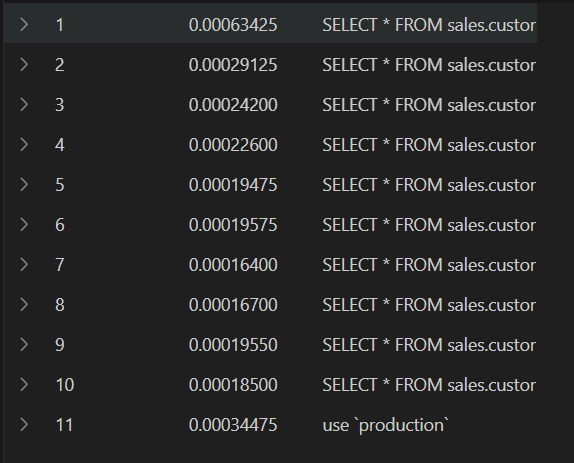
\includegraphics[width=0.75\linewidth]{figures//Nhân/mysql_brand_id.png}
    \caption{Kết quả thực hiện trong 10 lần với mySQL (đơn vị s)}
    \label{fig:indexing-1}
\end{figure}


\vspace{1em}

\noindent\textbf{2. Thực thi và đo lường trên Redis (In-memory NoSQL)}

Do Redis là cơ sở dữ liệu dạng \textit{Key-Value} không có lược đồ
(\textit{Schema-less}), để tìm kiếm sản phẩm theo \textit{Brand}, nhóm đã
thiết kế một cấu trúc \textit{Set} đóng vai trò như một \textit{Secondary Index}.
Key được đặt theo định dạng:

\texttt{production:products:brand:9}

chứa danh sách ID của các sản phẩm thuộc thương hiệu này.

\vspace{0.5em}

\noindent\textit{Câu lệnh truy xuất:}
\begin{lstlisting}[language=Python, basicstyle=\ttfamily\small, breaklines=true, frame=single]
SMEMBERS production:products:brand:9
\end{lstlisting}

\noindent\textit{Phương pháp đo lường:}

Nhóm sử dụng lệnh \texttt{CONFIG RESETSTAT} để làm sạch bộ đếm thống kê,
sau đó thực thi truy vấn nhiều lần. Kết quả thời gian trung bình được
trích xuất thông qua lệnh \texttt{INFO COMMANDSTATS}
(thông số \textit{usec\_per\_call}).

\vspace{0.5em}

\noindent\textbf{Kết luân Test Case 1}

\textbf{Thời gian thực thi trung bình:} khoảng \textasciitilde 0.016 ms
(16.3 micro-giây).

Do Redis lưu trữ toàn bộ dữ liệu trực tiếp trên bộ nhớ chính
(\textit{RAM}) và thao tác tìm kiếm trên cấu trúc \textit{Set} có độ phức tạp
$O(N)$ (với $N$ là số phần tử trả về), truy vấn gần như không phát sinh
độ trễ \textit{I/O} vật lý.

\begin{figure} [H]
    \centering
    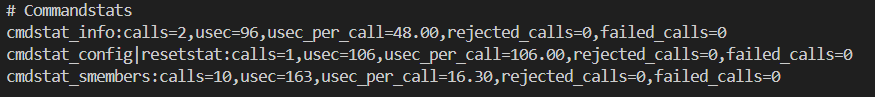
\includegraphics[width=0.75\linewidth]{figures//Nhân/redis_brand_id.png}
    \caption{Kết quả thực hiện trong 10 lần với Redis (đơn vị s)}
    \label{fig:indexing-2}
\end{figure}


\subsubsection{Test Case 2 — Tìm sản phẩm theo khoảng giá (MySQL có index, Redis không có)}


Mô tả kịch bản kiểm thử: Đánh giá hiệu năng xử lý truy vấn lọc dữ liệu theo một khoảng giá trị liên tục.

\begin{itemize}
    \item Dữ liệu sử dụng: Bảng products (321 sản phẩm)
    \item Yêu cầu: Tìm tất cả các sản phẩm có giá niêm yết list\_price nằm trong khoảng từ \$1000 đến \$2000.
\end{itemize}

\vspace{1em}

\noindent\textbf{1. Thực thi và Cơ chế trên MySQL (Relational Database)}

Trước hết, thực thi truy vấn (không có Index):

\begin{lstlisting}[language=Python, basicstyle=\ttfamily\small, breaklines=true, frame=single]
SELECT * FROM production.products 
WHERE list_price BETWEEN 1000 AND 2000;
\end{lstlisting}

Truy vấn được chạy 10 lần và lấy giá trị trung bình.

\textbf{Kết quả:} Thời gian thực thi trung bình khoảng \textasciitilde 0.76 ms.

\begin{figure} [H]
    \centering
    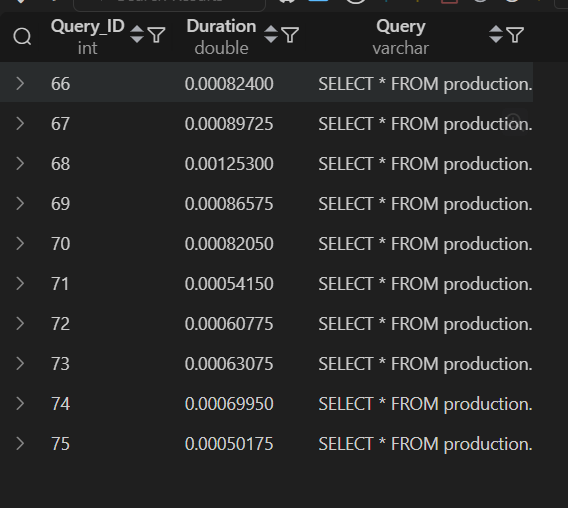
\includegraphics[width=0.75\linewidth]{figures//Nhân/mysql_test2.png}
    \caption{Kết quả thực hiện trong 10 lần với mySQL không index (đơn vị s)}
    \label{fig:indexing-3}
\end{figure}

\vspace{0.5em}

Sau đó, tiến hành tạo chỉ mục phụ (\textit{Secondary Index}) trên cột
\texttt{list\_price}:

\begin{lstlisting}[language=Python, basicstyle=\ttfamily\small, breaklines=true, frame=single]
CREATE INDEX idx_products_price 
ON production.products(list_price);
\end{lstlisting}

Tiếp tục chạy truy vấn 10 lần và tính trung bình.

\textbf{Kết quả:} Thời gian thực thi trung bình giảm xuống còn
\textasciitilde 0.56 ms.

\begin{figure} [H]
    \centering
    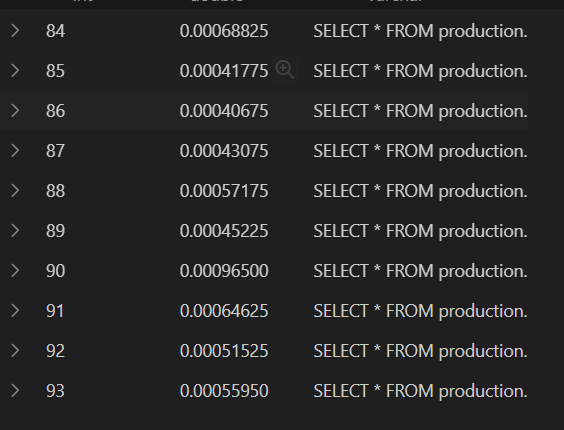
\includegraphics[width=0.75\linewidth]{figures//Nhân/mysql_test2_index.png}
    \caption{Kết quả thực hiện trong 10 lần với mySQL có indexing (đơn vị s)}
    \label{fig:indexing-4}
\end{figure}

\vspace{0.5em}

\noindent\textbf{Phân tích cơ chế xử lý}

Việc đánh chỉ mục đã giúp truy vấn nhanh hơn khoảng 26\%.

Khi chưa có Index, MySQL buộc phải thực hiện \textit{Full Table Scan}
(quét toàn bộ bảng) để kiểm tra từng dòng.

Khi có Index, MySQL chuyển sang sử dụng \textit{Index Range Scan}.
Cấu trúc cây \textit{B-Tree} đã sắp xếp sẵn các mức giá, giúp hệ thống
tìm nhanh đến điểm bắt đầu (\$1000) và duyệt dọc theo các nút lá
(\textit{leaf nodes}) cho đến khi đạt ngưỡng \$2000, từ đó loại bỏ
các dữ liệu không liên quan.

Mặc dù tập dữ liệu thử nghiệm khá nhỏ (321 dòng), sự chênh lệch hiệu năng
đã thể hiện rõ. Độ phức tạp thuật toán giảm từ $O(N)$ xuống còn
$O(\log N + M)$.

\vspace{1em}

\noindent\textbf{2. Thực thi và đo lường trên Redis (In-memory NoSQL)}

Do cấu trúc \textit{Hash} và \textit{Set} cơ bản của Redis không hỗ trợ
\textit{Range Index}, hệ thống buộc phải quét toàn bộ danh sách sản phẩm.

\begin{lstlisting}[language=Python, basicstyle=\ttfamily\small, breaklines=true, frame=single]
local pids = redis.call('SMEMBERS', 'production:products:ids')
local result = {}
for _, pid in ipairs(pids) do
    local price = tonumber(redis.call('HGET', 
        'production:product:' .. pid, 'list_price'))
    if price >= 1000 and price <= 2000 then
        local name = redis.call('HGET', 
            'production:product:' .. pid, 'product_name')
        table.insert(result, pid .. ' | ' .. name .. ' | $' .. price)
    end
end
return result
\end{lstlisting}

\vspace{0.5em}

\noindent\textbf{Kết quả đo lường}

Sử dụng lệnh \texttt{INFO COMMANDSTATS}, với chỉ số
\textit{usec\_per\_call} từ \texttt{cmdstat\_eval}, thời gian thực thi
trung bình ghi nhận được là 4{,}02 micro-giây.

\begin{figure} [H]
    \centering
    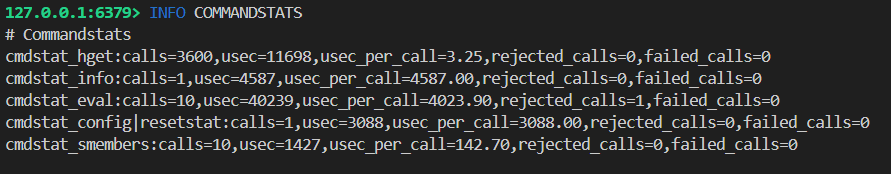
\includegraphics[width=0.75\linewidth]{figures//Nhân/redis_test2.png}
    \caption{Kết quả thực hiện trong 10 lần với redis (đơn vị s)}
    \label{fig:indexing-5}
\end{figure}

\vspace{0.5em}



\noindent\textbf{Phân tích cơ chế xử lý}

Mặc dù hoạt động hoàn toàn trên bộ nhớ chính (\textit{RAM}), Redis lại cho
thời gian phản hồi chậm hơn đáng kể so với MySQL. Nguyên nhân chính nằm ở
độ phức tạp thuật toán $O(N)$ và số lượng thao tác truy xuất rời rạc.

Cụ thể, hệ thống phải lấy toàn bộ 321 ID sản phẩm, sau đó duyệt qua từng
ID và thực hiện lệnh \texttt{HGET} 321 lần để kiểm tra giá
(\texttt{list\_price}).

Có 39 sản phẩm thỏa mãn điều kiện, do đó hệ thống tiếp tục thực hiện thêm
39 lệnh \texttt{HGET} để lấy tên sản phẩm (\texttt{product\_name}).

Tổng cộng, Redis phải thực hiện 360 thao tác truy xuất \textit{Hash}
rời rạc để hoàn thành truy vấn này.


\vspace{0.5em}

\noindent\textbf{Kết luận Test Case 2}

Đối với các bài toán truy vấn theo khoảng giá trị (\textit{Range Queries}),
hệ quản trị cơ sở dữ liệu quan hệ như \textbf{MySQL} với cấu trúc
\textit{B-Tree Index} thể hiện sự tối ưu vượt trội về mặt thuật toán.

Ngược lại, khi sử dụng kiến trúc \textit{Key-Value} cơ bản của Redis,
hệ thống buộc phải thực hiện quét toàn bộ tập dữ liệu
(\textit{Full Scan}), từ đó làm suy giảm đáng kể lợi thế tốc độ của việc
lưu trữ trên bộ nhớ \textit{RAM}.

Khi quy mô dữ liệu tăng lên hàng triệu bản ghi, thời gian truy vấn của Redis
(khi sử dụng Lua script) sẽ tăng tuyến tính theo độ phức tạp $O(N)$ và có
thể gây nghẽn luồng xử lý. Trong khi đó, MySQL vẫn duy trì hiệu năng ổn định
nhờ cấu trúc cây phân nhánh với độ phức tạp $O(\log N + M)$.



\subsubsection{Test Case 3 — Tìm sản phẩm theo tên (LIKE / pattern matching)}  ~\\
% Để một dòng trống hoàn toàn ở đây
\vspace{0.5em}


\noindent\textbf{Mô tả kịch bản kiểm thử}: Đánh giá hiệu năng khi xử lý dữ liệu có tính chất quan hệ, yêu cầu trích xuất
và tổng hợp thông tin từ nhiều thực thể khác nhau.

\textit{Yêu cầu:} Lấy danh sách toàn bộ sản phẩm (\texttt{Product ID, Name, Price})
kèm theo tên thương hiệu (\texttt{Brand Name}) và danh mục
(\texttt{Category Name}).

\textit{Thực thể tham gia:} \texttt{products}, \texttt{brands}, \texttt{categories}.

\textit{Đặc điểm:} Kiểm tra khả năng liên kết dữ liệu giữa các bảng (MySQL)
và khả năng truy xuất chéo khóa (Redis).

\vspace{1em}

\noindent\textbf{1. Thực thi và đo lường trên MySQL (Relational Database)}

\textit{Câu lệnh truy vấn:}
\begin{lstlisting}[language=SQL, basicstyle=\ttfamily\small, breaklines=true, frame=single]
SELECT 
    p.product_id, 
    p.product_name, 
    b.brand_name, 
    c.category_name, 
    p.list_price
FROM production.products p
JOIN production.brands b ON p.brand_id = b.brand_id
JOIN production.categories c ON p.category_id = c.category_id;
\end{lstlisting}

\textit{Kết quả đo lường:} Thời gian thực thi dao động từ
0.00044 đến 0.00071 giây, trung bình khoảng \textasciitilde 0.56 ms.

\begin{figure} [H]
    \centering
    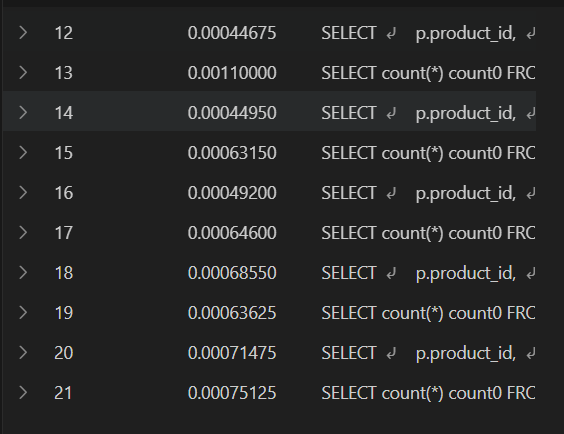
\includegraphics[width=0.75\linewidth]{figures//Nhân/mysql_test3.png}
    \caption{Kết quả thực hiện trong 10 lần với MySQL (đơn vị s)}
    \label{fig:indexing-6}
\end{figure}

\vspace{0.5em}

\noindent\textbf{Phân tích cơ chế xử lý}

MySQL được thiết kế tối ưu cho các thao tác quan hệ. Bộ tối ưu hóa truy vấn
(\textit{Query Optimizer}) tự động lựa chọn thuật toán kết nối phù hợp
(\textit{Nested-Loop Join}, \textit{Hash Join}) và tận dụng các chỉ mục
(\textit{Index}) trên khóa chính/khóa ngoại để ánh xạ dữ liệu hiệu quả
trong \textit{Buffer Pool}.

\vspace{1em}

\noindent\textbf{2. Thực thi và đo lường trên Redis (In-memory NoSQL)}

\textit{Cấu trúc và cách thực hiện:}

Do Redis không hỗ trợ phép \texttt{JOIN}, hệ thống phải tự thực hiện logic
kết nối bằng \textit{Lua Script}:

\begin{lstlisting}[language=bash, basicstyle=\ttfamily\small, breaklines=true, frame=single]
local pids = redis.call('SMEMBERS', 'production:products:ids')
local result = {}
for _, pid in ipairs(pids) do
    local p_key = 'production:product:' .. pid
    local pname = redis.call('HGET', p_key, 'product_name')
    local price = redis.call('HGET', p_key, 'list_price')
    local bid = redis.call('HGET', p_key, 'brand_id')
    local cid = redis.call('HGET', p_key, 'category_id')
    
    local bname = 'Unknown'
    if bid then 
        bname = redis.call('HGET', 'production:brand:' .. bid, 'brand_name') 
    end
    
    local cname = 'Unknown'
    if cid then 
        cname = redis.call('HGET', 'production:category:' .. cid, 'category_name') 
    end
    
    table.insert(result, pid .. ' | ' .. pname .. ' | ' .. bname .. 
        ' | ' .. cname .. ' | $' .. price)
end
return result
\end{lstlisting}

\vspace{0.5em}

\noindent\textbf{Kết quả đo lường}

Sau 10 lần thực thi, chỉ số \textit{usec\_per\_call} của
\texttt{cmdstat\_eval} ghi nhận khoảng 1{,}442.30 micro-giây
(\textasciitilde 1.44 ms).


\begin{figure} [H]
    \centering
    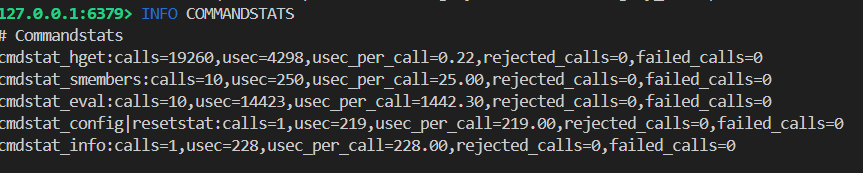
\includegraphics[width=0.75\linewidth]{figures//Nhân/redis_test3.png}
    \caption{Kết quả thực hiện trong 10 lần với Redis (đơn vị s)}
    \label{fig:indexing-7}
\end{figure}


\vspace{0.5em}

\noindent\textbf{Phân tích cơ chế xử lý}

Redis bộc lộ hạn chế rõ rệt khi xử lý dữ liệu quan hệ hóa
(\textit{Normalized Data}). Theo thống kê, hệ thống phải thực hiện
19{,}260 lệnh \texttt{HGET} trong 10 lần chạy thử.

Cụ thể:
\begin{itemize}
\item Lấy thông tin sản phẩm: 4 lệnh \texttt{HGET}
\item Lấy tên thương hiệu: 1 lệnh \texttt{HGET}
\item Lấy tên danh mục: 1 lệnh \texttt{HGET}
\end{itemize}

Tổng cộng 6 lệnh \texttt{HGET} cho mỗi sản phẩm. Với 321 sản phẩm,
Redis cần thực hiện 1{,}926 thao tác truy xuất cho mỗi lần chạy.

Mặc dù hoạt động trên \textit{RAM}, số lượng thao tác lớn và việc xử lý
chuỗi khiến hiệu năng tổng thể bị suy giảm đáng kể.


\noindent\textbf{Kết luận Test Case 3:} Đối với các bài toán có tính chất quan hệ phức tạp và yêu cầu tổng hợp dữ liệu từ nhiều thực thể (JOIN), MySQL là sự lựa chọn không thể thay thế. Redis sinh ra không phải để giải quyết bài toán nối bảng. Việc cố gắng ép Redis chạy các truy vấn quan hệ thông qua vòng lặp ở tầng ứng dụng (hoặc Lua Script) sẽ gây ra hiệu ứng N+1 Query, làm tiêu tốn lượng lớn tài nguyên CPU để tra cứu từng Khóa rời rạc, khiến nó chậm hơn cả việc truy xuất từ đĩa cứng có đệm của cơ sở dữ liệu quan hệ truyền thống.



\subsubsection{Test case 4: Tìm đơn hàng theo điều kiện phức hợp (Composite Condition)}

\vspace{0.5em}

\noindent\textbf{Mô tả kịch bản kiểm thử}

Đánh giá khả năng xử lý của hệ quản trị khi người dùng yêu cầu lọc dữ liệu dựa trên nhiều điều kiện (\textit{AND}) cùng lúc.

\textit{Dữ liệu sử dụng:} \texttt{sales.orders}.

\textit{Yêu cầu:} Tìm tất cả đơn hàng thuộc chi nhánh \texttt{store\_id = 1}, 
đã hoàn thành (\texttt{order\_status = 4}) và được tạo trong năm 2017 
(từ \texttt{2017-01-01} đến \texttt{2017-12-31}).

\vspace{1em}

\noindent\textbf{1. Thực thi và đo lường trên MySQL (Relational Database)}

\textit{Câu lệnh truy vấn:}

\begin{lstlisting}[language=SQL, basicstyle=\ttfamily\small, breaklines=true, frame=single]
SELECT * FROM sales.orders 
WHERE store_id = 1 AND order_status = 4 
AND order_date BETWEEN '2017-01-01' AND '2017-12-31';
\end{lstlisting}

\textit{Kết quả đo lường:} Thời gian thực thi dao động từ 0.00061 đến 0.00142 giây, 
trung bình khoảng \textasciitilde 0.96 ms.


\begin{figure} [H]
    \centering
    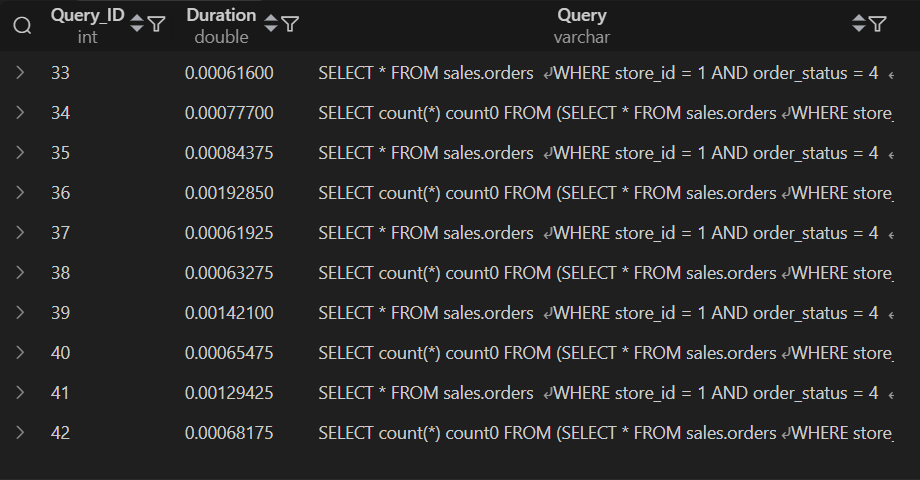
\includegraphics[width=0.75\linewidth]{figures//Nhân/mysql_test4.png}
    \caption{Kết quả thực hiện trong 10 lần với MySQL (đơn vị s)}
    \label{fig:indexing-8}
\end{figure}



\vspace{0.5em}

\noindent\textbf{Phân tích cơ chế xử lý}

MySQL xử lý các điều kiện phức hợp hiệu quả nhờ \textit{Query Optimizer}. 
Ngay cả khi chưa có \textit{Composite Index}, hệ thống vẫn có thể tận dụng 
các chỉ mục đơn để khoanh vùng dữ liệu, sau đó áp dụng bộ lọc trực tiếp.

\vspace{1em}

\noindent\textbf{2. Thực thi và đo lường trên Redis (In-memory NoSQL)}

\textit{Cấu trúc và cách thực hiện:}

Redis không hỗ trợ \texttt{JOIN} hoặc truy vấn đa điều kiện trực tiếp, do đó 
cần sử dụng chiến lược \textit{Two-step Filtering} bằng Lua Script.

\begin{lstlisting}[language=bash, basicstyle=\ttfamily\small, breaklines=true, frame=single]
local oids = redis.call('SMEMBERS', 'sales:orders:store:1')
local result = {}
for _, oid in ipairs(oids) do
    local status = redis.call('HGET', 'sales:order:' .. oid, 'order_status')
    local date = redis.call('HGET', 'sales:order:' .. oid, 'order_date')
    if status == '4' and date >= '2017-01-01' and date <= '2017-12-31' then
        table.insert(result, oid .. ' | ' .. date .. ' | status=' .. status)
    end
end
return result
\end{lstlisting}

\vspace{0.5em}

\noindent\textbf{Kết quả đo lường}

Sau 10 lần thực thi, chỉ số \textit{usec\_per\_call} ghi nhận thời gian 
trung bình khoảng 1{,}678.30 micro-giây (\textasciitilde 1.68 ms).


\begin{figure} [H]
    \centering
    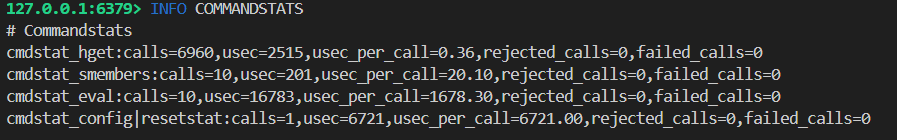
\includegraphics[width=0.75\linewidth]{figures//Nhân/redis_test4.png}
    \caption{Kết quả thực hiện trong 10 lần với Redis (đơn vị s)}
    \label{fig:indexing-9}
\end{figure}


\vspace{0.5em}

\noindent\textbf{Phân tích cơ chế xử lý}

Redis phải thực hiện nhiều thao tác \texttt{HGET} rời rạc. Trung bình mỗi lần chạy,
script gọi khoảng 696 lần đọc \textit{Hash}, tương ứng với khoảng 348 đơn hàng.

Chiến lược dùng \textit{Set} để thu hẹp phạm vi tìm kiếm đã cải thiện hiệu năng, 
tuy nhiên việc truy xuất dữ liệu rời rạc vẫn là nút thắt cổ chai.

\vspace{1em}

\noindent\textbf{Kết luận Test Case 4}

MySQL cho thấy sự ổn định và dễ triển khai với truy vấn đa điều kiện nhờ cú pháp 
khai báo và cơ chế tối ưu hóa mạnh mẽ. Redis có thể xử lý tốt nếu thiết kế dữ liệu 
phù hợp, nhưng với các truy vấn phức tạp nhiều điều kiện, mô hình quan hệ vẫn chiếm 
ưu thế rõ rệt so với kiến trúc \textit{Key-Value}.


\subsection{Tạo Sorted Set index trong Redis}

\vspace{1em}

\noindent\textbf{Tối ưu Test Case 2 trên Redis với Sorted Set (ZSET)}

Ở Test Case 2 (tìm sản phẩm theo khoảng giá), việc sử dụng \textit{Hash} và
\textit{Set} cơ bản khiến Redis phải thực hiện \textit{Full Scan} với độ phức tạp
$O(N)$, dẫn đến thời gian thực thi chậm (\textasciitilde 4.02 ms) so với
MySQL (\textasciitilde 0.56 ms).

Để khắc phục hạn chế này, nhóm triển khai \textit{Secondary Index} trên Redis
bằng cấu trúc dữ liệu \textit{Sorted Set (ZSET)}.

\vspace{0.5em}

\noindent\textbf{Nguyên lý xây dựng chỉ mục}

Mỗi phần tử trong ZSET gồm:
\begin{itemize}
\item \textbf{Score:} Giá trị \texttt{list\_price}
\item \textbf{Member:} \texttt{product\_id}
\end{itemize}

\vspace{0.5em}

\noindent\textbf{Bước 1: Khởi tạo chỉ mục}

\begin{lstlisting}[language=bash, basicstyle=\ttfamily\small, breaklines=true, frame=single]
EVAL "
local pids = redis.call('SMEMBERS', 'production:products:ids')
for _, pid in ipairs(pids) do
    local price = tonumber(redis.call('HGET', 
        'production:product:' .. pid, 'list_price'))
    redis.call('ZADD', 'production:products:by_price', price, pid)
end
return redis.call('ZCARD', 'production:products:by_price')
" 0
\end{lstlisting}

\vspace{0.5em}

\noindent\textbf{Bước 2: Truy vấn khoảng giá}

Thay vì sử dụng vòng lặp, Redis cung cấp lệnh chuyên dụng:

\begin{lstlisting}[language=SQL, basicstyle=\ttfamily\small, breaklines=true, frame=single]
ZRANGEBYSCORE production:products:by_price 1000 2000
\end{lstlisting}

\vspace{0.5em}

\noindent\textbf{Kết quả đo lường}

Sau khi thực hiện \texttt{CONFIG RESETSTAT} và chạy truy vấn 10 lần,
chỉ số \textit{usec\_per\_call} từ \texttt{cmdstat\_zrangebyscore}
ghi nhận thời gian trung bình khoảng 571.40 micro-giây
(\textasciitilde 0.57 ms). Nhanh hơn nhiều so với thực hiện \textit{Full Scan} (\textasciitilde 4.02 ms)

\begin{figure} [H]
    \centering
    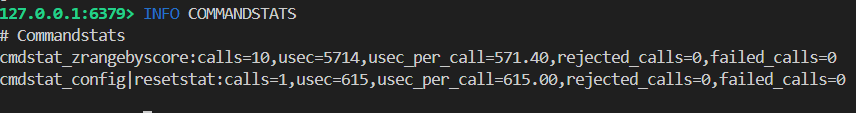
\includegraphics[width=0.75\linewidth]{figures//Nhân/redis_sorted.png}
    \caption{Kết quả thực hiện trong 10 lần với Redis (đơn vị micro-giây)}
    \label{fig:indexing-10}
\end{figure}

\vspace{0.5em}

\noindent\textbf{Nhận xét}

Cấu trúc \textit{ZSET} được xây dựng dựa trên thuật toán
\textit{Skip List} kết hợp với \textit{Hash Table}. Khi sử dụng
\texttt{ZRANGEBYSCORE}, Redis có thể truy cập trực tiếp đến phần tử có
giá trị \texttt{score} bắt đầu (1000), sau đó duyệt tuần tự đến mốc
2000.

Điều này giúp độ phức tạp giảm từ $O(N)$ xuống $O(\log N + M)$.
Kết quả là hiệu năng truy vấn của Redis (\textasciitilde 0.57 ms)
đã gần tương đương với MySQL (\textasciitilde 0.56 ms) khi sử dụng
\textit{B-Tree Index}.


\subsection{Kết luận}


\begin{table}[htpb]
\centering
\renewcommand{\arraystretch}{1.5} % Tăng khoảng cách giữa các hàng cho thoáng
\begin{tabular}{|p{3.5cm}|p{4.2cm}|p{4.5cm}|p{3.2cm}|}
\hline
\textbf{Test Case} & \textbf{MySQL} & \textbf{Redis} & \textbf{Ghi chú (Kết luận)} \\ \hline
Tìm theo FK (brand\_id) & Nhanh ($\sim$0.20 ms) \newline \textit{(Dùng B-Tree Index)} & \textbf{Rất nhanh ($\sim$0.016 ms)} \newline \textit{(Dùng Set O(1) trên RAM)} & \textbf{Redis thắng} \\ \hline
Range query (giá) & \textbf{Nhanh ($\sim$0.56 ms)} \newline \textit{(Dùng B-Tree Index Range Scan)} & Chậm ($\sim$4.02 ms) \newline \textit{(Phải Full Scan bằng Lua script)} & \textbf{MySQL thắng} \\ \hline
Truy vấn kết nối (JOIN) & \textbf{Nhanh ($\sim$0.56 ms)} \newline \textit{(Hỗ trợ native, tối ưu sâu)} & Chậm ($\sim$1.44 ms) \newline \textit{(Bị lỗi N+1 query, quét thủ công)} & \textbf{MySQL thắng}  \\ \hline
Composite condition & \textbf{Nhanh ($\sim$0.96 ms)} \newline \textit{(Query Optimizer tự kết hợp)} & Khá chậm ($\sim$1.68 ms) \newline \textit{(Dùng Set pre-filter + filter vòng lặp)} & \textbf{MySQL thắng}  \\ \hline
\end{tabular}
\caption{Kết quả thực tế đo lường so sánh hiệu năng giữa MySQL và Redis}
\label{tab:mysql_vs_redis_results}
\end{table}


Mặc dù phiên bản Redis tiêu chuẩn (Core Redis) bộc lộ hạn chế khi xử lý truy vấn khoảng (Range Query) và đa điều kiện (Composite Condition) do phải quét dữ liệu tuần tự (với độ phức tạp $O(N)$), hệ sinh thái Redis cung cấp một giải pháp khắc phục triệt để mang tên \textbf{RediSearch}. 

Đây là một module mở rộng chính thức, biến Redis thành một công cụ tìm kiếm mạnh mẽ bằng cách tự động hóa việc tạo chỉ mục thứ cấp (Secondary Indexing) và hỗ trợ cấu trúc \textit{Inverted Index} tối ưu. 

Thay vì phải tự viết các đoạn mã (\textit{Lua Script}) lặp qua từng phần tử một cách thủ công, RediSearch cho phép thực hiện các truy vấn đa điều kiện và tìm kiếm toàn văn (\textit{Full-text Search}) chỉ với một câu lệnh duy nhất. 

Việc tích hợp RediSearch trong thực tế sẽ giúp hệ thống triệt tiêu hoàn toàn nút thắt cổ chai $O(N)$, đưa tốc độ truy vấn phức tạp về mức dưới 1 mili-giây, giúp Redis vừa giữ được sức mạnh \textit{In-memory}, vừa linh hoạt không kém gì các hệ quản trị cơ sở dữ liệu quan hệ truyền thống.



